\documentclass[smaller]{beamer}

\usepackage{helvet}
\usepackage{hyperref, graphicx}
\usepackage{amsthm}
\usepackage{amsfonts}
\usepackage{etoolbox}
\usepackage{wrapfig}
\usepackage{tikz}
\usepackage{ulem}
\usepackage{fontspec}
%\usepackage[T1]{fontenc}
%\setmainfont{Cambria}
%\usefonttheme{serif}

\usetheme{default}
\setbeamertemplate{navigation symbols}{}
\AtBeginSection[ ]
{
\begin{frame}{Outline}
    \tableofcontents[currentsection]
\end{frame}
}

% Default fixed font does not support bold face
\DeclareFixedFont{\ttb}{T1}{txtt}{bx}{n}{11} % for bold
\DeclareFixedFont{\ttm}{T1}{txtt}{m}{n}{12}  % for normal - use in headings

% Custom colors
\usepackage{color}
\definecolor{TUGray}{RGB}{101,101,137}
\definecolor{TUBlack}{RGB}{30,0,0}
\definecolor{mygreen}{RGB}{45,111,63}
\definecolor{keywords}{RGB}{205,114,0}
\definecolor{comments}{RGB}{181,51,139}
\definecolor{strings}{RGB}{58,144,81}
\definecolor{numeric}{RGB}{66,110,176}
\definecolor{linos}{rgb}{0.4,0.4,0.4}
\definecolor{links}{rgb}{0,0.4,0.75}

\definecolor{bggray}{RGB}{232, 233, 235}

\usecolortheme[named=mygreen]{structure}
\setbeamercolor{normal text}{fg=TUBlack}\usebeamercolor*{normal text}

\setbeamercolor{codecol}{fg=TUGray!25!black,bg=bggray}

\hypersetup{colorlinks, linkcolor=links, urlcolor=links}



\usepackage[sfdefault,scaled=.85]{FiraSans}
\usepackage{newtxsf}

\usepackage{listings}

\newtoggle{InString}{}% Keep track of if we are within a string
\togglefalse{InString}% Assume not initally in string

\newcommand\digitstyle{\color{numeric}}
\makeatletter
\newcommand{\ProcessDigit}[1]
{%
  \ifnum\lst@mode=\lst@Pmode\relax%
   {\digitstyle #1}%
  \else
    #1%
  \fi
}
\makeatother

\lstset{literate=%
    {0}{{{\ProcessDigit{0}}}}1
    {1}{{{\ProcessDigit{1}}}}1
    {2}{{{\ProcessDigit{2}}}}1
    {3}{{{\ProcessDigit{3}}}}1
    {4}{{{\ProcessDigit{4}}}}1
    {5}{{{\ProcessDigit{5}}}}1
    {6}{{{\ProcessDigit{6}}}}1
    {7}{{{\ProcessDigit{7}}}}1
    {8}{{{\ProcessDigit{8}}}}1
    {9}{{{\ProcessDigit{9}}}}1
	{<=}{{\(\leq\)}}1
	{>=}{{\(\geq\)}}1,
	% morestring=[b]",
    % morestring=[b]',
    % morecomment=[l]{//},
}

\lstdefinelanguage{Pseudo}{
    morekeywords={return, while, if, for, input},
    morecomment=[l]{\#},
}

% Pseudocode style
\newcommand\pseudostyle{\lstset{
language=Pseudo,
basicstyle=\fontfamily{ccr}\scriptsize,
commentstyle=\it\scriptsize\color{linos},
keywordstyle=\it\bfseries\scriptsize,
mathescape=true,
literate=
    {=}{$\leftarrow{}$}{1}
    {==}{$={}$}{1}
    {<=}{{\(\leq\)}}1
	{>=}{{\(\geq\)}}1,
xleftmargin=18pt,
xrightmargin=4pt,
aboveskip=12pt,
belowskip=0pt,
frame=tB,
keepspaces=true
}}

% Python style for highlighting
\newcommand\pythonstyle{\lstset{
language=Python,
basicstyle=\ttfamily\tiny,
numbers=left,
numberstyle=\tiny\color{linos},
morekeywords={self, np},              % Add keywords here
keywordstyle=\tiny\color{keywords},
commentstyle=\it\tiny\color{comments},    % Custom highlighting style
stringstyle=\tiny\color{strings},
xleftmargin=18pt,
xrightmargin=4pt,
aboveskip=0pt,
belowskip=0pt,
escapeinside={(*@}{@*)},
frame=l,                         % Any extra options here
showstringspaces=false,
keepspaces=true
}}

% Pseudocode environment
\lstnewenvironment{pseudo}[1][]
{
    \pseudostyle
    \lstset{
        #1
    }
}
{}

% Python environment 
\lstnewenvironment{python}[1][]
{
	\pythonstyle
	\lstset{
	#1
	}
}
{}

% wrap the Python environment
\newenvironment{codeblock}
    {\hfill\begin{beamerboxesrounded}[lower=codecol, width=0.8\textwidth]
    \medskip

    }
    { 
    \end{beamerboxesrounded}\hfill
    }

\theoremstyle{example}
\newtheorem{question}{Question}

\newcommand{\ct}[1]{\lstinline[language=Python]!#1!}
\newcommand{\ttt}[1]{{\small\texttt{#1}}}
\newcommand{\lsitem}[2]{\ttt{{#1}[}\ct{#2}\ttt{]}}

\newcommand{\x}{\textbf{x}}
\newcommand{\ix}[1]{{\it #1}}

\author{Chris Cornwell}
\date{April 15, 2025}
\title{Diagnostics for Choosing a Model}

\begin{document}

\begin{frame}
\titlepage
\end{frame}

\begin{frame}
    \frametitle{Outline}
    \tableofcontents
\end{frame}

\section{Making choices about your model}

%%%%
\begin{frame}
\frametitle{Intro}
Previously, discussed the Bias-Variance trade-off and making a careful choice of hypothesis class of functions that, for your data, does not exhibit too much Bias, nor too much Variance.

\pause
Given our type of machine learning model, what are properties that can be ``tuned'' to change the Bias and Variance? 
\pause
\begin{itemize}
    \item Initial, but not perfect, answer is the total number of parameters (i.e., the numbers, or \textit{weights}, that are updated by the procedure which, from training data $\mathcal S$, determines $f_S$). Sometimes, more of these parameters \texttt{=} higher Variance, but this is not definitive and depends on other choices and model type.
    \pause
    \item After determining the type of model, choices are made before training that affect both the hypothesis class and training procedure. These are \textbf{hyperparameters}. Examples of hyperparameters:
    \begin{enumerate}
        \pause
        \item For a decision tree model: the \lstinline[language=Python,basicstyle=\ttfamily]{max_depth} of the tree.
        \pause
        \item For a neural network model: the number of \ttt{hidden layers} in the network.
        \pause
        \item For a support vector machine: the type of kernel that is used {--} e.g., if you will use a polynomial kernel and the \ttt{degree} of the polynomial kernel.
        \pause
        \item For clustering: for $K$-means clustering, the number \ttt{K}; for \ttt{DBSCAN} clustering, the radius \ttt{epsilon}.
    \end{enumerate}
\end{itemize}

\end{frame}

%%%%
\begin{frame}
    \frametitle{Choosing Hyperparameters}
How do you choose the hyperparameters?

\pause
As always, first split your data into training data and test data.\footnote{Don't touch the test data until the model, with parameters, is trained and ready to perform on data.} Common splits of training and test data are 70/30 percent or 80/20 percent for training/test (not a ``hard and fast'' rule).

\pause
One method: a \textbf{grid search}. Say that you have $M$ hyperparameters. Further, say that for the $j^{th}$ hyperparameter you have chosen a ``reasonable'' range of values, such that $N_j$ values of the hyperparameter are possible.\footnote{In particular, if the hyperparameter is real-valued, then you have picked a partition (or step-size) in the interval. For example, $0.0, 0.05, 0.1, \ldots, 0.95, 1.0$ in interval $[0,1]$.}

\pause
Let $\mathcal L_{test}$ be the loss value on the test data. The set of all possible $M$-tuples of hyperparameters has size $\prod_{j=1}^M N_j$. A grid search method is to train a model for each of the possible $M$-tuples and then compute $\mathcal L_{test}$. Then, you choose the model with the smallest $\mathcal L_{test}$ value.

\pause
\textbf{Downsides:} most notably, as described it \textit{uses the test data} to make a decision about the parameters. Can potentially cause overfitting. \newline 
It is also typically computationally expensive.
\end{frame}

%%%%
\begin{frame}
    \frametitle{Validation Sets}
In addition to splitting the data into a training set and test set, it is common practice to have an additional split of the training set, with some amount put into a \textbf{validation set}. 

\pause
The validation data may then be used to assess how good the hyperparameter choices are {--} computing the loss on validation data, $\mathcal L_{valid}$ say {--} and we are able to keep the test data locked away until the end, for assessment of the final model.

\pause
For example, a grid search method might be applied, but choosing the model with smallest $\mathcal L_{valid}$, rather than $\mathcal L_{test}$, and this will help the $\mathcal L_{test}$ of the final model be a better estimate of the expected population loss.
\end{frame}

\section{High Bias vs.\ High Variance}

%%%%
\begin{frame}
    \frametitle{Diagnostic to Test for High Bias}
    Use validation data to diagnose if chosen hyperparameters create too much Bias or too much Variance. 
    \vfill 

    \pause
    \begin{itemize}
        \item In training/validation/test split of data, say that $n$ is the number of points in training subset. For a series of values of $m$ with $m\le n$, train a model with your choice of hyperparameters, with just $m$ of points from training data. Then, compute the value of $\mathcal L_{train}$ and $\mathcal L_{valid}$ on each of the resulting models.

        \pause
        \item Plot the curves for $\mathcal L_{train}$ and $\mathcal L_{valid}$, as functions of $m$. In a scenario with high Bias, they appear as depicted below. Note that the $\mathcal L_{train}$ and $\mathcal L_{valid}$ curves approach each other as $m$ increases; however, the loss (even on training data) is too high. 
    \end{itemize}

    \begin{figure}
        \begin{center}
        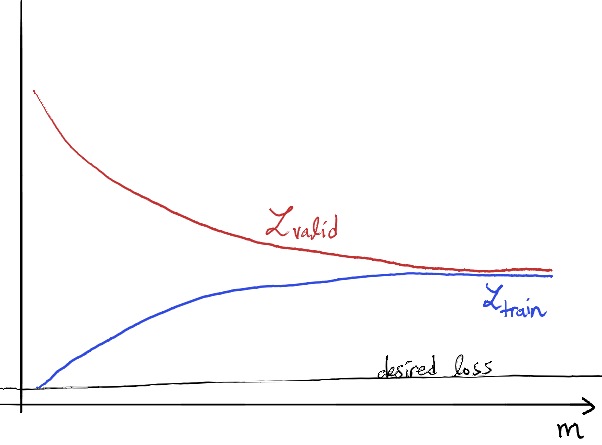
\includegraphics[height=0.3\textheight]{../../Images/high-bias-schematic.png}
        \end{center}
        \caption{High Bias Scenario; m is the \# of data points used in training.}
    \end{figure}
\end{frame}

%%%%
\begin{frame}
    \frametitle{Diagnostic to Test for High Variance}
    \begin{itemize}
        \item However, if $\mathcal L_{train}$ and $\mathcal L_{valid}$ are computed as before, and their curves plotted as functions of $m$, then in a scenario with high Variance, they will appear as depicted below. Here, between the $\mathcal L_{train}$ and $\mathcal L_{valid}$ curves there is a gap, that remains as $m$ increases. 
    \end{itemize}

    \begin{figure}
        \begin{center}
            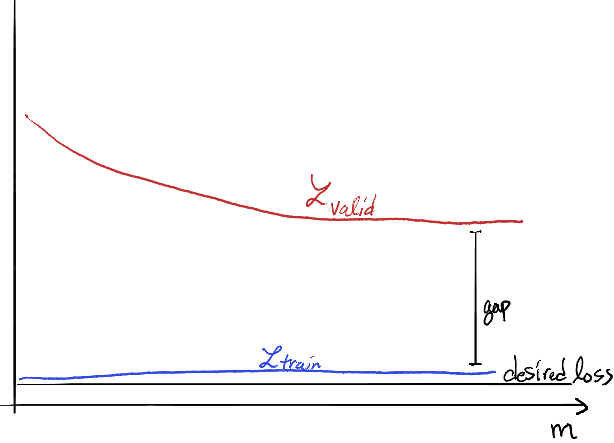
\includegraphics[height=0.3\textheight]{../../Images/high-variance-schematic.png}
        \end{center}
        \caption{High Variance Scenario; $m$ is the \# of data points used in training.}
    \end{figure}

    \pause
    In practice, the curves are not so smooth; e.g., the order in which training points are added (as $m$ increases) to the training set has an effect on getting low training (or validation) loss score. 
    \pause
    \begin{itemize}
        \item To see the above shape, may need to randomly re-order the training data multiple times, redo the computations, and plot the averages as the curve.
    \end{itemize}
\end{frame}

%%%%
\begin{frame}
    \frametitle{Diagnostic for high Bias versus high Variance}
    Recall from last lecture, the decision tree (with no maximum depth) which was fit to classify the digit in a handwritten image. 

    Below, the diagnostic was run when setting the maximum depth of the tree equal to 2. The curve is indicative of the Bias being high. The number of points in the training set is along the horizontal axis. \footnote{Remark: for this data, the log loss value shown for training data meant that less than 50\% of the images were being classified correctly.}

    \pause
    \centering 
    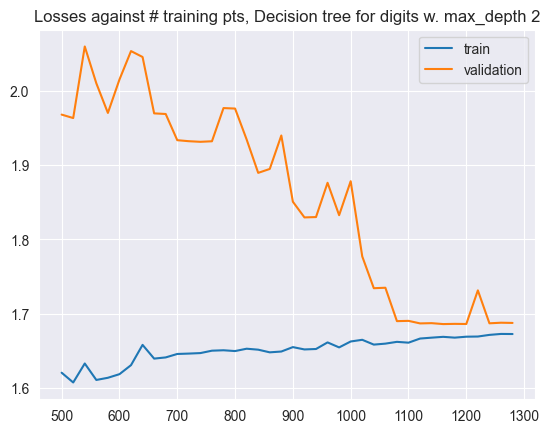
\includegraphics[height=0.45\textheight]{../../Images/high-bias-Tree-DigitsImages.png}
\end{frame}


%%%%
\begin{frame}
    \frametitle{Diagnostic for high Bias versus high Variance}
    The same diagnostic was run, but setting the maximum depth of the tree equal to 10. The curve is shown below and is indicative of a scenario when Variance is high.

    \vfill

    \centering 
    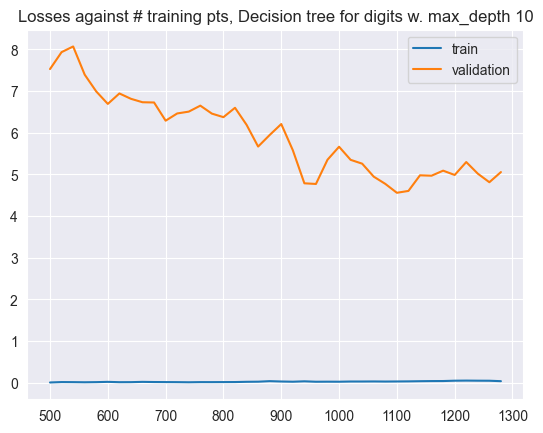
\includegraphics[width=0.6\textwidth]{../../Images/high-variance-Tree-DigitsImages.png}
\end{frame}

\section{Cross-Validation}

%%%%
\begin{frame}[fragile]
    \frametitle{Cross-Validation}
    If you are not in a ``data rich'' setting {--} that is, you do not have a large amount of data {--} then setting aside 10-20\% of it as validation data might make it difficult to train a model that performs well. Additionally, \textit{which} data goes into the validation subset might affect the resulting prediction function, and its performance, significantly.
    
    A remedy is to use $k$-fold \textbf{cross-validation}. Commonly, practitioners use 5-fold or 10-fold cross-validation. Here, we describe the 5-fold version. 

    After having separated out the test data, randomly sort your remaining data into 5 subsets. For example, if \ttt{x} is the array to be separated into 5 arrays, the following would do the job.

\begin{codeblock}

\begin{python}
indices = np.arange(len(x))
np.random.shuffle(indices)
n_subset = int(len(x)/5)
for i in range(5):
    subsets[i] = x[i*n_subset:(i+1)*n_subset]
\end{python}

\end{codeblock}

Next, you train and do validation on 5 models, with training sets determined from the subsets:

\begin{center}
    \begin{tabular}{|c|c|c|c|c|}
        \hline 
        train & train & train & train & valid \\ 
        \hline
        \hline
        train & train & train & valid & train \\ 
        \hline
        \hline
        train & train & valid & train & train \\ 
        \hline
        \hline
        train & valid & train & train & train \\ 
        \hline
        \hline
        valid & train & train & train & train \\
        \hline
    \end{tabular}
\end{center}
\end{frame}

\end{document}